\chapter[Descrição do Processo]{Descrição do Problema/Processo ou O Processo de Fazer Alguma Coisa}
\label{chap:descricaoproblema}
%Note que, como nome do capítulo é muito longo, fornecemos um nome abreviado uso no cabeçalho

Se desejar, uma visão geral do capítulo pode ser colocada antes da primeira seção. Este é o capítulo de descrição do processo e formulação do problema. Tendo em vista que se trata de uma monografia de engenharia de controle e automação, em muitos casos será fundamental a apresentação dos sensores e atuadores do processo.


\section{Processo de Fazer Alguma Coisa}
\label{sec:hist}

Cada seção inicia pela descrição do seu conteúdo e pode terminar com um parágrafo de conexão com a seção seguinte. 

Antes de formular o problema, \textbf{não se esqueça de fazer todas as definições necessárias}. Também devem-se detalhar os aspectos complementares da abordagem: se estamos estudando um aspeto particular do problema, se a resposta encontrada é universal ou dependente de simplificações e hipóteses prévias.


\section{Instrumentação do Processo}
\label{sec:instrumentação}

Descreva a aparelhagem e o equipamento utilizados bem como a ligação entre os diversos componentes. Nesta seção e, ao longo de todo o texto, você deve dar detalhes suficientes para que qualquer pessoa consiga reproduzir seus experimentos.

Contudo, \textbf{não disperse o leitor com detalhes irrelevantes} ou aspectos
demasiado técnicos ou formais. Reserve tais detalhes para um
apêndice.

Como uma imagem vale mais que mil palavras, e como usar mil palavras prejudicaria a clareza do texto, ilustramos o processo com a Figura \ref{fig:processo}. Lembrar que toda figura deve ser comentada no texto, você nunca deve colocar figuras que fiquem ``soltas'' no texto.  

\begin{figure}[thpb]
  \centering
  \resizebox{120mm}{!}{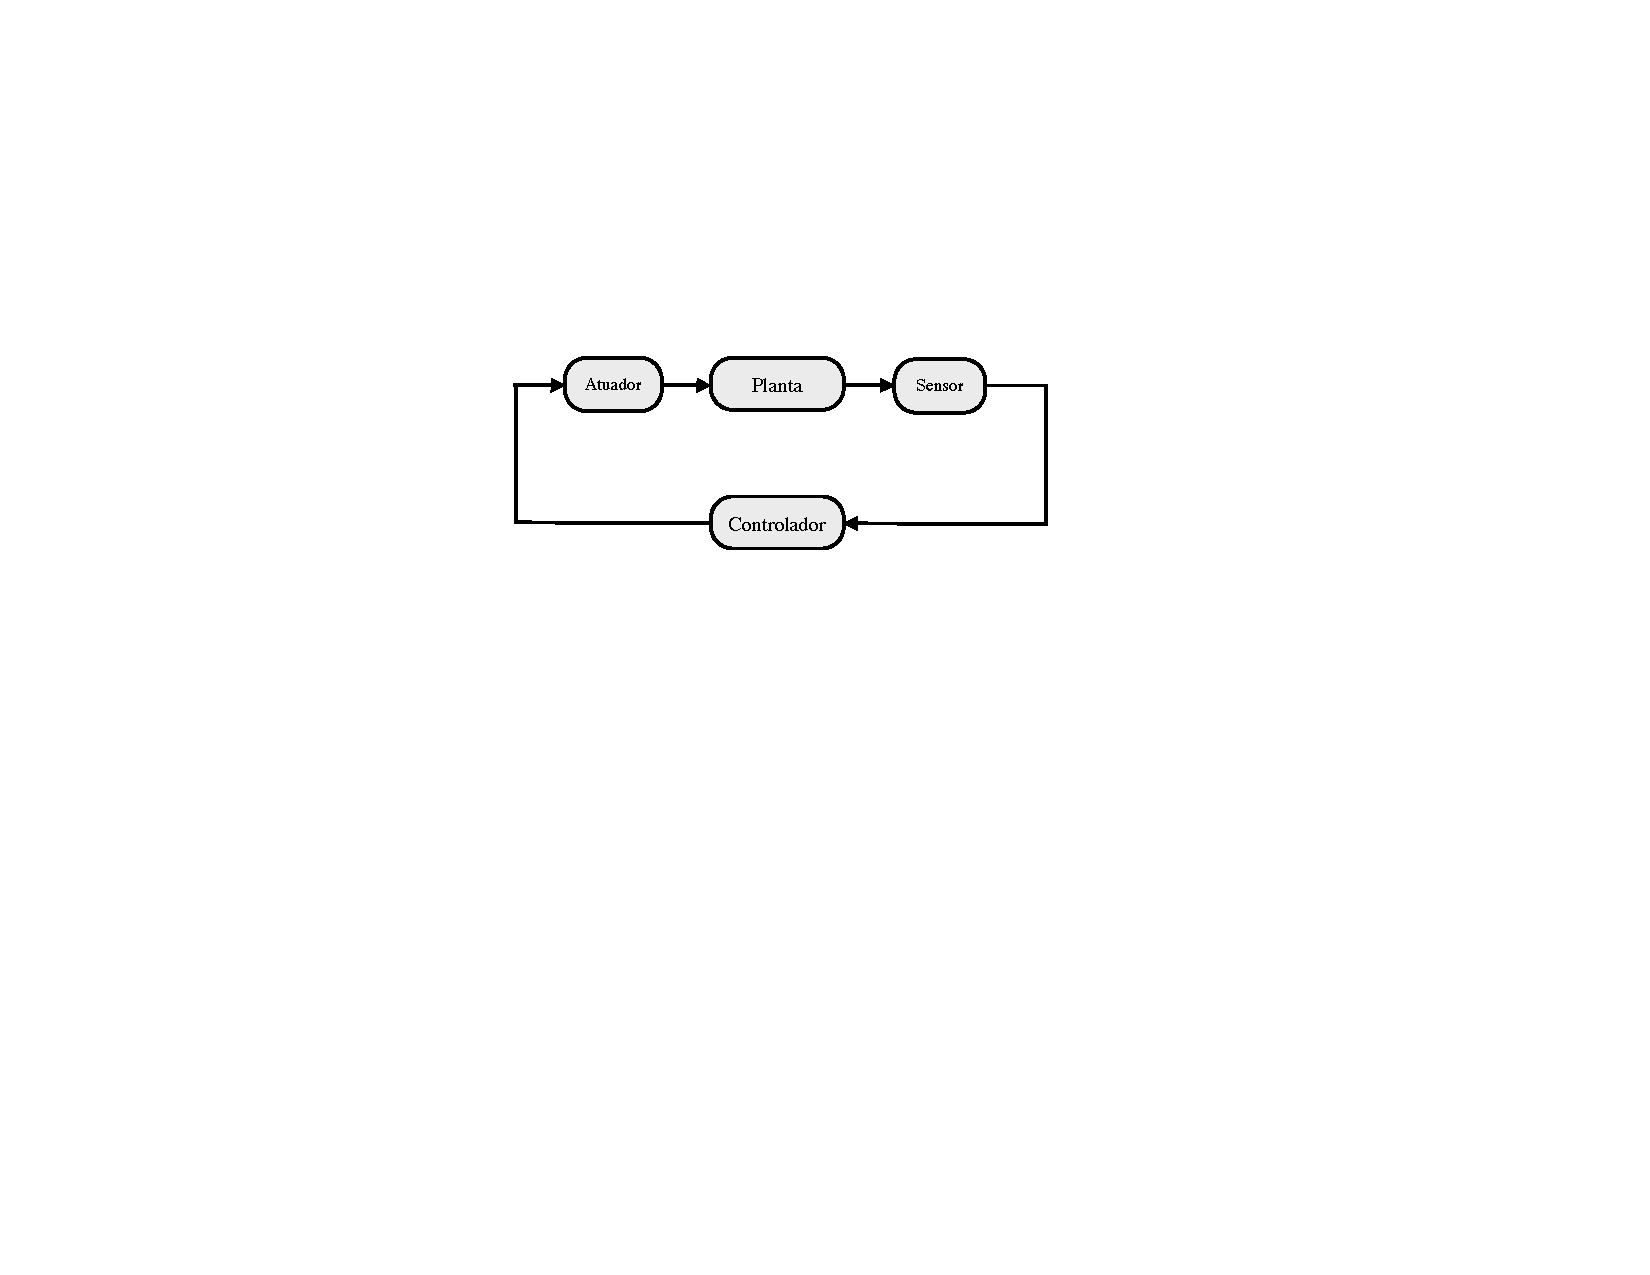
\includegraphics{DescricaoProcesso/Figuras/FiguraProcesso.pdf}}
  \caption{Aqui escrevemos \textbf{toda} informação pertinente à figura. Ou seja, este texto deve ser uma descrição auto-contida da figura, não sendo necessário recorrer ao corpo de texto para saber detalhes sobre a mesma. \emph{Fonte:} Citar fonte se figura 	não for elaborada pelo autor e \textbf{pedir permissão para usar!}}
  \label{fig:processo}
\end{figure}


\section{Situação Atual/Estado da Arte/Revisão da Literatura}
\label{sec:revisão}

Este é o espaço para uma revisão detalhada do enquadramento do problema. Isso inclui descrever a situação atual do processo, aquilo que foi feito até então dentro da empresa/laboratório, e aquilo que se pode chamar de ``Estado da Arte'', ou seja, uma apresentação do conhecimento preexistente
sobre o tema do projeto.

A elaboração desta seção tipicamente demanda uma boa revisão da literatura. Deve haver, quando aplicável uma análise das soluções potencialmente concorrentes, elencando vantagens e desvantagens.

\subsection{Como Elaborar uma Revisão da Literatura}

Ao selecionar referências, devem-se preferir referências de veículos confiáveis, que tenham por exemplo processo de revisão por pares. Portanto, dá-se preferência a artigos em periódicos e livros, em seguida teses e dissertações, artigos em anais de congresso e por fim relatórios. Evitar citar páginas da internet por oferecem menor garantia da informação nelas contida. 

Pesquise sua bibliografia em bases confiáveis como o \textsf{Web of Science}, \textsf{Scopus}, ou o \textsf{Google Scholar}. \textbf{Não use uma ferramenta de busca comum!} (elas não foram feitas pensando no \emph{ranking} de textos científicos) Use o número de citações de uma dada referência como um indicador de sua qualidade. Explore os artigos que citam a referência estudada bem como os artigos que ela cita.

Prefira as referências mais recentes quando se tratar de um assunto na fronteira do conhecimento ou de tecnologia de ponta. Quando se tratar de um assunto já consolidado, prefira citar livros ou artigos com muitas citações. 

Evite citar informações de segunda-mão e procure na medida do possível rastrear a fonte original. Contudo, em situações em que a fonte original é de acesso mais difícil, seja por ter tido publicação limitada como no caso de relatórios ou por não ser em língua inglesa ou portuguesa, é preferível a citação de segunda-mão em um veículo mais acessível.

Para gerenciar suas referências, use uma ferramenta de software como o \textsf{Mendeley}, que permite gerar arquivos .bib para uso em {\LaTeX} ou simplesmente gerar a lista de referências para uso direto em editores de texto. Em \LaTeX, mais especificamente Bib\TeX, a lista de referências é criada a partir de um arquivo .bib, que é uma espécie de banco de informações bibliográficas em que cada entrada é uma referência associada a uma chave para citação. A lista criada incluirá apenas as referências citadas ao longo do texto, mesmo que haja mais referências no arquivo .bib. As informações bibliográficas no formato Bib\TeX também podem ser obtidas para cada referência em ferramentas como o \textsf{Google Scholar} e então coladas no arquivo .bib.

Na Seção \ref{sec:comocitar} discutiremos como e quando as citações devem ser usadas.

\section{Resumo do Capítulo}

Tente não terminar de forma abrupta. Se for escrever algo aqui, não seja genérico!


\clearpage
